\subsection{Mission d'AMO~: Présentation de \mo}

\subsubsection{Présentation de \mo}
\begin{frame}
	\frametitle {Présentation de \mo} 
	\begin{block}{Présentation générale} \pause
		\begin{itemize}
			\item L'une des plus grandes organisations humanitaires au monde \pause
			\item Agit avant, pendant et après les catastrophes et les urgences relatives à la santé \pause
			\item Puise sa force de son réseau de volontaires
		\end{itemize}
	\end{block}
\end{frame}

%% Présentation de Gk et de son projet.
% Gestion de la planification, du suivi, documentaire.
\begin{frame}
	\frametitle {Présentation de \mo} \pause
	\begin{figure}[htbp]
		\centering
		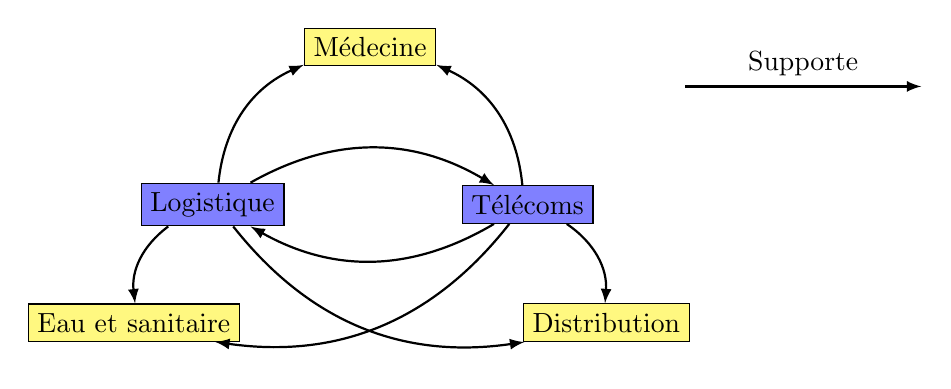
\begin{tikzpicture}
			% définition des styles
			\tikzstyle{metier}=[rectangle,draw,fill=yellow!50,text=black]
			\tikzstyle{support}=[rectangle,draw,fill=blue!50,text=black]
			\tikzstyle{supporte}=[->,>=latex,thick,rounded corners=4pt]
			% les nœuds
			\node[metier] (e) at (-3,-3) {Eau et sanitaire};
			\node[metier] (m) at (0,0.5) {Médecine};
			\node[metier] (d) at (3,-3) {Distribution};
			\node[support] (l) at (-2,-1.5) {Logistique};
			\node[support] (t) at (2,-1.5) {Télécoms};
			% les flèches
			\draw[supporte] (l) to[bend left] (t);
			\draw[supporte] (l) to[bend right] (e);
			\draw[supporte] (l) to[bend left] (m);
			\draw[supporte] (l) to[bend right] (d);
			\draw[supporte] (t) to[bend left] (l);
			\draw[supporte] (t) to[bend left] (e);
			\draw[supporte] (t) to[bend right] (m);
			\draw[supporte] (t) to[bend left] (d);
			% la légende
			\draw[supporte] (4,0) -- (7,0) node[midway,above]{Supporte};
		\end{tikzpicture}
		\caption{Dépendances entre les métiers}
	\end{figure}  
\end{frame}

\subsubsection{Présentation du projet}
\begin{frame}
	\frametitle {Présentation de \mo} \pause
	\begin{block}{Processus de la logistique} \pause
		\begin{enumerate}
			\item Achat \pause
			\item Stockage \pause
			\item Transport
		\end{enumerate}
	\end{block}
	\begin{block}{Fonctions clefs de la logistique} \pause
		\begin{enumerate}
			\item Planification/évaluation \pause
			\item Acquisition/achat \pause
			\item Gestion des entrepôts \pause
			\item Organisations des transports \pause
			\item Suivi et compte rendu
		\end{enumerate}
	\end{block}
\end{frame}

\subsubsection{Objectifs du projet}
\begin{frame}
	\frametitle {Présentation de \mo} 
	\begin{block}{Objectifs de la mission d'AMO pour \mo}
		\begin{itemize}
			\item Améliorer la qualité de ses services en se dotant d'une solution de type Transport Management System(TMS) 
			\item Espérance de retour sur investissement
		\end{itemize}
	\end{block}
\end{frame}

\begin{frame}
	\frametitle {Présentation de \mo} 
	\begin{figure}[htbp] % Arbre à problèmes
		\centering
			\begin{tikzpicture} [
					node distance = 0.4cm, auto,font=\footnotesize,
					% STYLES
					every node/.style={node distance=1.7cm},
					% The comment style is used to describe the characteristics of each force
					comment/.style={rectangle, inner sep= 3pt, text width=2.8cm, node distance=0.2cm, font=\scriptsize\sffamily},
					% The force style is used to draw the forces' name
					force/.style={rectangle, draw, fill=black!10, inner sep=3pt, text width=2.8cm, text badly centered, minimum height=1cm, font=\bfseries\normalsize\sffamily}
				]
				% Nodes
				\node [force] (confiance) {Confiance\\{\normalfont\footnotesize Envers \mo}};
				\node [force, above of=confiance] (transparent) {Transparence des informations\\{\normalfont\footnotesize Grâce au suivi détaillé}};
				%% Mj %% Bug avec 'X[cm] of transparent' -> Mise ne commentaire et réécriture sans
				\node [force, right=0.6cm of transparent] (serieux) {Sérieux\\{\normalfont\footnotesize Car on peut justifier à tout moment de l'utilisation des ressources}};
				\node [force, left=0.6cm of transparent] (pro) {Professionnalisme\\{\normalfont\footnotesize Notamment grâce à la planification et à l'utilisation optimale du matériel}};
				\node [force, below of=confiance, left=-0.2cm of confiance] (don) {Dons à l'organisation};
				\node [force, below of=confiance, right=-0.2cm of confiance] (benevolat) {Hausse du bénévolat};
%				\node [force, right] (serieux) {Sérieux\\{\normalfont\footnotesize Car on peut justifier à tout moment de l'utilisation des ressources}};
%				\node [force, left] (pro) {Professionnalisme\\{\normalfont\footnotesize Notamment grâce à la planification et à l'utilisation optimale du matériel}};
%				\node [force, below of=confiance, left] (don) {Dons à l'organisation};
%				\node [force, below of=confiance, right] (benevolat) {Hausse du bénévolat};
				% Draw the links between forces
				\path[->,thick]
					(don) edge (confiance)
					(benevolat) edge (confiance)
					(confiance) edge (transparent)
					(confiance) edge (serieux)
					(confiance) edge (pro);
			\end{tikzpicture} 
		\caption{Arbre à problème : Finalité du projet et retour sur investissement}
	\end{figure}
\end{frame}

\begin{frame}
	\frametitle {Présentation de \mo}
	\begin{block}{Nature des prestations demandées}
		\mo recherche  un prestataire pour la réalisation d'une solution TMS, les prestations attendues ~:
		\begin{enumerate}
			\item la suite logicielle \pause
			\item le matériel \pause
			\item le service support
		\end{enumerate}
	\end{block} \pause
	\begin{block}{Parties concernées}
		\begin{enumerate}
			\item Directement: les logisticiens de \mo
			\item Indirectement: les victimes prises en charge
		\end{enumerate}
	\end{block}
\end{frame}

\begin{frame}
	\frametitle {}
\end{frame}
